\documentclass[tikz,border=2pt]{standalone}
\usepackage{tikz}
\usetikzlibrary{arrows.meta,fit,positioning,backgrounds}
\definecolor{navy}{HTML}{2F5D8C}
\definecolor{teal}{HTML}{14866D}
\definecolor{orange}{HTML}{D98200}
\definecolor{purple}{HTML}{7556A3}
\definecolor{red}{HTML}{B84444}
\definecolor{ink}{HTML}{24313D}
\definecolor{pblue}{HTML}{EAF2F8}
\definecolor{pteal}{HTML}{E8F5F1}
\definecolor{porange}{HTML}{FFF3DE}
\definecolor{ppurple}{HTML}{F1ECF8}
\begin{document}
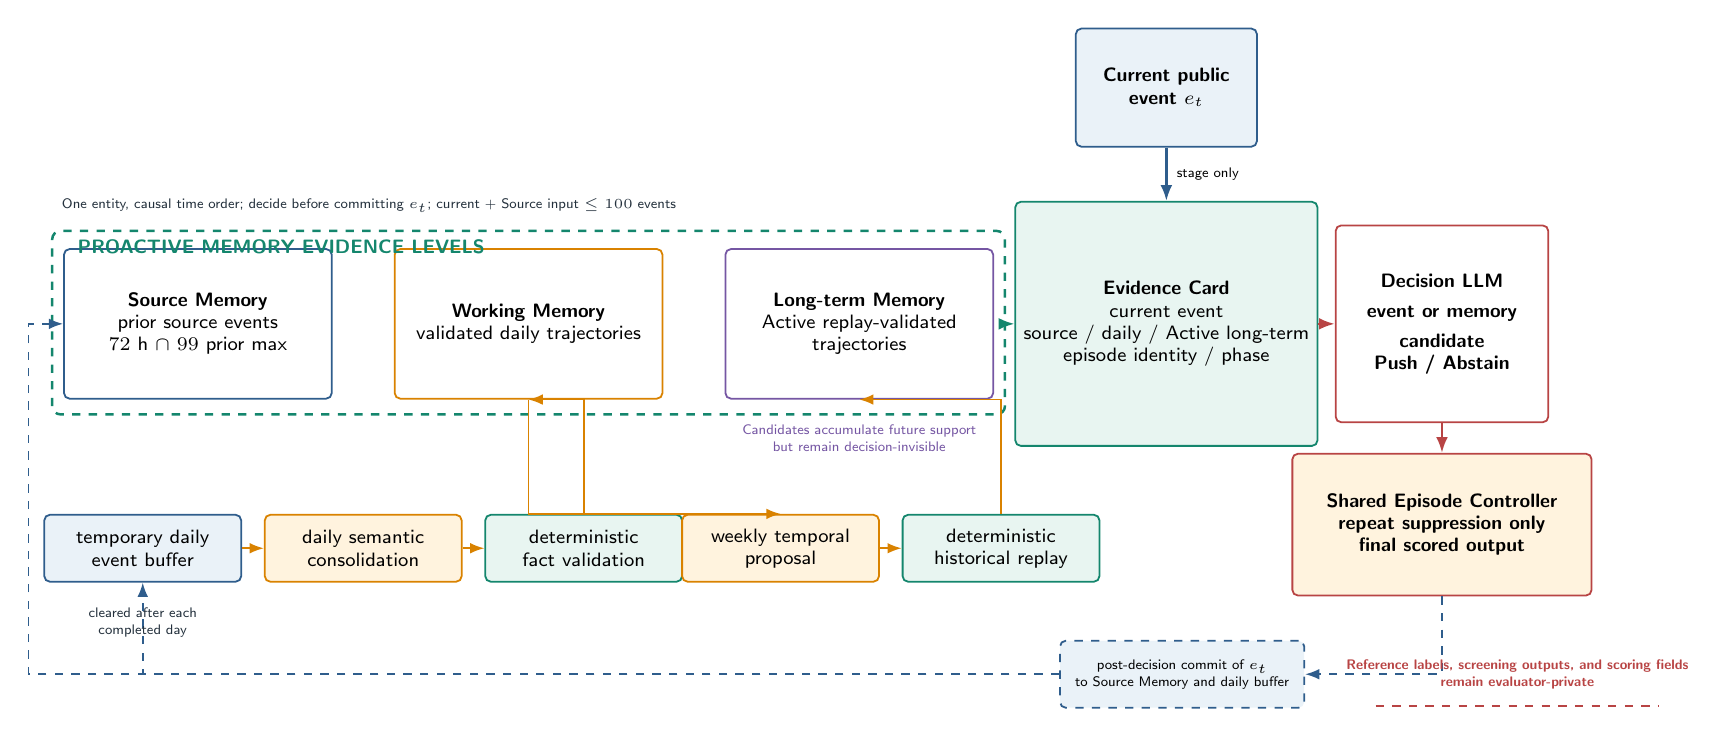
\begin{tikzpicture}[
  font=\sffamily\scriptsize,
  box/.style={rounded corners=2pt,draw=ink,line width=.65pt,fill=white,align=center,minimum height=8.5mm,inner sep=3pt},
  arrow/.style={-{Latex[length=2mm]},line width=.75pt,draw=ink},
  maintenance/.style={-{Latex[length=1.8mm]},line width=.65pt,draw=orange},
  postwrite/.style={-{Latex[length=1.8mm]},line width=.65pt,draw=navy,dashed},
  sectiontitle/.style={font=\sffamily\bfseries\scriptsize,anchor=west}
]
\node[box,draw=navy,minimum width=34mm,minimum height=19mm] (source) at (3.3,1.2) {\textbf{Source Memory}\\prior source events\\$72$ h $\cap$ $99$ prior max};
\node[box,draw=orange,minimum width=34mm,minimum height=19mm] (working) at (7.5,1.2) {\textbf{Working Memory}\\validated daily trajectories};
\node[box,draw=purple,minimum width=34mm,minimum height=19mm] (longterm) at (11.7,1.2) {\textbf{Long-term Memory}\\Active replay-validated\\trajectories};
\draw[teal,dashed,rounded corners=3pt,line width=.9pt] (1.45,.05) rectangle (13.55,2.38);
\node[sectiontitle,text=teal] at (1.65,2.18) {PROACTIVE MEMORY EVIDENCE LEVELS};

\node[box,draw=navy,fill=pblue,minimum width=25mm] (buffer) at (2.6,-1.65) {temporary daily\\event buffer};
\node[box,draw=orange,fill=porange,minimum width=25mm] (daily) at (5.4,-1.65) {daily semantic\\consolidation};
\node[box,draw=teal,fill=pteal,minimum width=25mm] (fact) at (8.2,-1.65) {deterministic\\fact validation};
\node[box,draw=orange,fill=porange,minimum width=25mm] (weekly) at (10.7,-1.65) {weekly temporal\\proposal};
\node[box,draw=teal,fill=pteal,minimum width=25mm] (replay) at (13.5,-1.65) {deterministic\\historical replay};

\draw[maintenance] (buffer) -- (daily);
\draw[maintenance] (daily) -- (fact);
\draw[maintenance] (fact.north) |- (working.south);
\draw[maintenance] (working.south) |- (weekly.north);
\draw[maintenance] (weekly) -- (replay);
\draw[maintenance] (replay.north) |- (longterm.south);

\node[box,draw=navy,fill=pblue,minimum width=23mm,minimum height=15mm,font=\sffamily\bfseries\scriptsize] (event) at (15.6,4.2) {Current public\\event $e_t$};
\node[box,draw=teal,fill=pteal,minimum width=34mm,minimum height=31mm] (card) at (15.6,1.2) {\textbf{Evidence Card}\\current event\\source / daily / Active long-term\\episode identity / phase};
\node[box,draw=red,fill=white,minimum width=27mm,minimum height=25mm,font=\sffamily\bfseries\scriptsize] (decision) at (19.1,1.2) {Decision LLM\\[1mm]event \emph{or} memory\\[1mm]candidate\\\textsc{Push / Abstain}};
\node[box,draw=red,fill=porange,minimum width=38mm,minimum height=18mm,font=\sffamily\bfseries\scriptsize] (controller) at (19.1,-1.35) {Shared Episode Controller\\repeat suppression only\\final scored output};
\node[box,draw=navy,fill=pblue,dashed,minimum width=31mm,font=\sffamily\tiny] (commit) at (15.8,-3.25) {post-decision commit of $e_t$\\to Source Memory and daily buffer};

\draw[arrow,draw=navy,line width=.9pt] (event.south) -- node[right,font=\sffamily\tiny]{stage only} (card.north);
\draw[arrow,draw=teal] (13.55,1.2) -- (card.west);
\draw[arrow,draw=red,line width=.9pt] (card) -- (decision);
\draw[arrow,draw=red,line width=.9pt] (decision.south) -- (controller.north);
\draw[postwrite] (controller.south) |- (commit.east);
\draw[postwrite] (commit.west) -- (1.15,-3.25) -- (1.15,1.2) -- (source.west);
\draw[postwrite] (commit.west) -- (2.6,-3.25) -- (buffer.south);

\node[font=\sffamily\tiny,align=center,text=ink,below=2mm of buffer] {cleared after each\\completed day};
\node[font=\sffamily\tiny,align=center,text=purple,below=2mm of longterm] {Candidates accumulate future support\\but remain decision-invisible};
\node[font=\sffamily\bfseries\tiny,align=center,text=red,right=4mm of commit] (private) {Reference labels, screening outputs, and scoring fields\\remain evaluator-private};
\draw[red,dashed,line width=.65pt] ([xshift=-18mm,yshift=-1mm]private.south) -- ([xshift=18mm,yshift=-1mm]private.south);
\node[font=\sffamily\tiny,text=ink,anchor=west] at (1.45,2.7) {One entity, causal time order; decide before committing $e_t$; current + Source input $\leq 100$ events};
\end{tikzpicture}
\end{document}
